\newif\ifvimbug
\vimbugfalse

\ifvimbug
\begin{document}
\fi

\exercise{Principle Component Analysis}
In this exercise you will use the \texttt{Iris.txt} dataset. It contains data from three kind of Iris flowers (`Setosa', `Versicolour' and `Virginica') with 4 attributes: sepal length, sepal width, petal length, and petal width. Each row contains a sample while the last attribute is the label. A label of $0$ means that the sample comes from a `Setosa' plant, $1$ from a `Versicolour', and $2$ from `Virginica'.
(You are allowed to use built-in functions for computing the mean, the covariance, eigevalues and eigenvectors.)

\begin{questions}

%----------------------------------------------

\begin{question}{Data Normalization}{4}
Normalizing the data is a common practice in machine learning. Normalize the provided dataset such as it has zero mean and unit variance per dimension. Why is normalizing important?
Attach a snippet of your code. 

\begin{answer}
Subtracting the mean of the dataset is important, because otherwise the results of the Principal component analysis would be meaningless. Normalizing for unit variance prevents variables with a large variance to influence the PCA too significantly.

The normalization is done by the following function:
\lstinputlisting[language=Python, firstline=11, lastline = 21]{../Code/33a.py}
	
\end{answer}

\end{question}

%----------------------------------------------

\begin{question}{Principle Component Analysis}{8}
Apply PCA on your normalized dataset and generate a table showing the proportion (percentage) of cumulative variance explained. 
How many components do you need in order to explain at least $95\%$ of the dataset variance? 
Attach a snippet of your code.

\begin{answer}
The Principal Component Analysis of a normalized dataset X can be computed using the following snippet:

\lstinputlisting[language=Python, firstline=25, lastline=28]{../Code/33a.py}



The cumulative explained variance of these Eigenvalues is 
\[
\begin{array}{c|c|c|c}
\lambda_1& \lambda_2 & \lambda_3 & \lambda_4 \\ \hline
0.72770452 & 0.95800975 & 0.99484807 & 1.
\end{array} 
\]

Therefore, in order to explain more than 95\% variance, 2 Eigenvectors are needed.
	
\end{answer}

\end{question}

%----------------------------------------------

\begin{question}{Low Dimensional Space}{6}
Using as many components as needed to explain $95\%$ of the dataset variance, generate a scatter plot of the lower-dimensional projection of the data. Use different colors or symbols for data points from different classes. 
What do you observe? Attach a snippet of your code.

\begin{answer}
The first step is to project the data. This is done by a simple dot-multiplication. In the snippet, the dataset is transposed because of the order of the data in the given file. The result is transposed to restore that order:
\lstinputlisting[language=Python, firstline=64, lastline=65]{../Code/33a.py}


The data is plotted using the following snippet, where C0, C1 and C2 indicate the samples that belong to the corresponding class:
\lstinputlisting[language=Python, firstline=67, lastline=74]{../Code/33a.py}

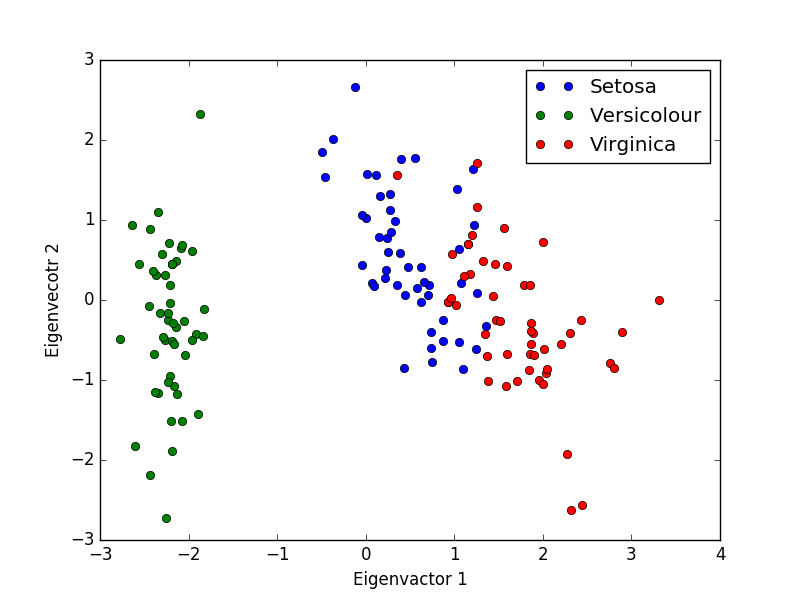
\includegraphics[width=1.0\linewidth]{./img/33c.png}

From this perspective, the plant Versicolour is easily separable from the other two plants. Setosa and Virginica are also separated, but they overlap.

\end{answer}

\end{question}

%----------------------------------------------

\begin{question}{Projection to the Original Space}{6}
Reconstruct the original dataset by using different number of principle components. Using the normalized root mean square error (NRMSE) as a metric, create a table with the error per input versus the amount of principle components used (i.e., with five columns: first for the number of components, remainder for the input NRMSE).
Attach a snippet of your code.
(Remember that in the first step you normalized the data.)


\begin{answer}


\[\begin{array}{lcccc}
	Components & 1 & 2 & 3 & 4 \\ 
	NRMSE & a & b & c & d
\end{array} 
\]
	
\end{answer}
\end{question}

\begin{question}[bonus]{Kernel PCA}{15}
Throughout this class we have seen that PCA is an easy and efficient way to reduce the dimensionality of some data. However, it is able to detect only linearly dependences among data points. A more sophisticated extension to PCA, \emph{Kernel PCA}, is able to overcome this limitation. 
This question asks you to deepen this topic by conducting some research by yourself: explain what Kernel PCA is, how it works and what are its main limitations. Be as much as concise (but clear) as possible.

\begin{answer}
The PCA decorrelates the features given in a dataset by diagonalizing the covariance matrix, given by 
\[S = \frac{1}{N} \sum_{n=1}^{N}x_n x_n^T\]
Unfortunately, this only works well, if the relation between the feature is linear.

To circumvent this problem, a transformation $\Phi (x)$ can be used to project the samples into a feature space. In an ideal feature space, the relations between two different features are only linear. Consider an example, where two features, $x_{(1)}$ and $x_{(2)}$ have a quadratic relationship: $x_{(2)} = 5 \cdot x_{(1)}^2$. A transformation $\Phi(x) = (\begin{matrix}
x_{(1)}^2\\
x_{(2)}
\end{matrix}) $ would make this relationship linear and therefore PCA applicable.

This means, that in Kernel PCA, the covariance matrix of the feature space 
\[S'=\frac{1}{N} \sum_{n=1}^{N} \Phi(x_n) \Phi(x_n)^T\]
is diagonalized by solving its eigenvector equation \[S'v_i = \lambda_i v_i\]

However, transforming every sample into the feature space by applying $\Phi(x)$ is a very computation intensive operation. Therefore, the goal is to solve this eigenvector problem without having to work in the feature space.  
 
\end{answer}

\end{question}

\end{questions}
